\textbf{תזכורת:}
כפל נאיבי של מטריצה בגודל 
$a \times b$
עם מטריצה בגודל 
$b \times c$
לוקח 
$O(a \cdot b \cdot c)$
פעולות.
התוצאה של המכפלה היא מטריצה מגודל 
$a \times c$.

כאשר כופלים $n$ מטריצות, 
$A_1,\ldots,A_n$
מגדלים 
$x_i \times y_i$
בהתאמה, אז תוצאת המכפלה תהיה מטריצה מגודל
$x_1 \times y_n$.
מספר הפעולות שיש לבצע תלוי בסדר בו נבחר לבצע את המכפלה.

\textbf{דוגמה:}
כמה פעולות נבצע כדי לבצע את המכפלה
$ABC$
?
$$
\begin{pmatrix}
a_{1}
\\
a_{2}
\\
\vdots
\\
a_{100}
\end{pmatrix}
%
\begin{pmatrix}
b_{1}	&	b_{2} & \dots &  b_{100}
\end{pmatrix}
%
\begin{pmatrix}
c_{1}
\\
c_{2}
\\
\vdots
\\
c_{100}
\end{pmatrix}
$$

אם נבצע את המכפלה לפי הסדר משמאל לימין אז נזדקק ל-%
$100 \cdot 1 \cdot 100 = 10,000$
פעולות עבור הכפל של 
$AB$
ו-%
$100 \cdot 1 \cdot 100 = 10,000$
פעולות נוספות עבור הכפל של
$(AB)C$.
אם נחשב את המכפלה
$A(BC)$
אז נזדקק לסדר גודל של 200 פעולות בלבד !!!

\textbf{בעיה:}
בהינתן $n$ מטריצות, 
$A_1,\ldots,A_n$
מגדלים 
$x_i \times y_i$
בהתאמה, רוצים לחשב סדר מכפלות שדורש מינימום פעולות.

\textbf{ייצוג סדר מכפלות}
ייצוג טבעי לסדר הפעולות הוא בעזרת עץ, למשל העץ הבא מתאים לחישוב
$(AB)(C((DE)F))$
:
\begin{center}
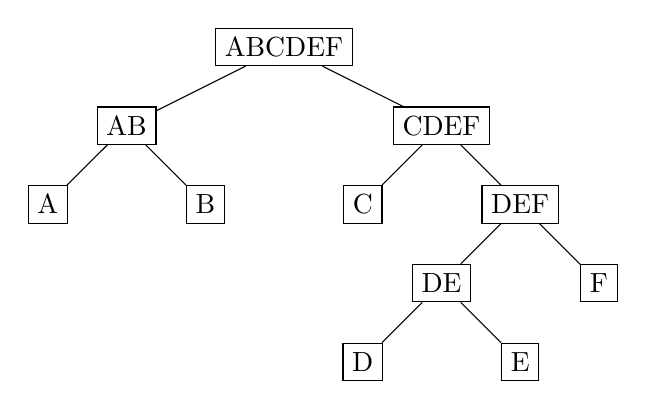
\begin{tikzpicture}[every node/.style={rectangle, draw}]
\foreach \x \y \t in {
	0/0/ABCDEF%
	,-2/-1/AB,2/-1/CDEF%
	,-3/-2/A,-1/-2/B%
	,1/-2/C,3/-2/DEF%
	,2/-3/DE,4/-3/F%
	,1/-4/D,3/-4/E%
}{
	\node(\t) at(\x,\y) {\t};
}

\foreach \u \v in {
	ABCDEF/AB,ABCDEF/CDEF%
	,AB/A,AB/B%
	,CDEF/C,CDEF/DEF%
	,DEF/DE,DEF/F%
	,DE/D,DE/E%
}{
	\draw (\u) -- (\v);
}
\end{tikzpicture}
\end{center}

נתייחס לעץ כזה כעץ ביטוי, עץ ביטוי הוא עץ בינרי מלא שבו העלים הם המטריצות מהקלט וכל צומת 
מייצג מכפלה של המטריצות המתאימות לעלים של תת העץ שלו.

\textbf{אלגוריתם:}
עבור כל 
$1 \leq i \leq j \leq n$
נגדיר את
$\alpha(i, j)$
להיות מספר הפעולות המינימלי שצריך כדי לבצע את המכפלה
$A_i \cdot A_{i + 1} \cdot \ldots \cdot A_j$

אז מתקיים ש:%
$$
\alpha(i, j) = \min_{i \leq k < j} 
\alpha(i, k) + \alpha(k + 1, j) + x_i \cdot y_k \cdot y_j
$$

בנוסף מתקיים ש:
$$
\forall \; 1 \leq i \leq n \; \alpha(i,i) = 0
$$

\textbf{סיבוכיות:}
אם מחשבים את ערכי נוסחת הנסיגה על ידי שימוש בטבלה, למשל, אז נדרש לחשב
$O(n^2)$
ערכים. 
זמן החישוב של כל ערך הוא 
$O(n)$
ולכן בסך הכל זמן ריצת האלגוריתם הוא:
$O(n^3)$.

\textbf{דוגמת הרצה:}
$$
A_1^{9 \times 2} A_2^{2 \times 10} A_3^{10 \times 4} A_4^{4 \times 3}
$$
